\documentclass[tikz,border=2pt]{standalone}
\usepackage{amsmath}
\usepackage{pgfplots}
\pgfplotsset{compat=1.18}

\begin{document}
% Polynomials of degree 1, 2 and 3: smooth everywhere, with at most "degree" many zeros and
% ends that run off to ±∞ according to the leading term.
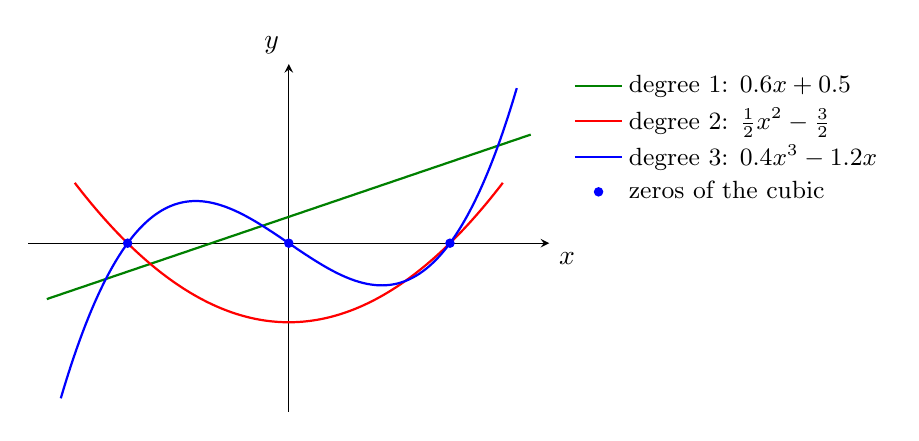
\begin{tikzpicture}
	\begin{axis}[
		axis lines=middle,
		xmin=-2.8, xmax=2.8,
		ymin=-3.2, ymax=3.4,
		xtick=\empty, ytick=\empty,
		xlabel={$x$}, ylabel={$y$},
		xlabel style={below right}, ylabel style={above left},
		samples=150, smooth, clip=false,
		width=8.2cm, height=6cm,
		legend pos=outer north east, legend style={draw=none, fill=none, font=\small}, legend cell align=left
		]
		\addplot[thick, green!50!black, domain=-2.6:2.6] {0.6*x+0.5};
		\addlegendentry{degree 1: $0.6x+0.5$}
		\addplot[thick, red, domain=-2.3:2.3] {0.5*x^2-1.5};
		\addlegendentry{degree 2: $\tfrac12x^2-\tfrac32$}
		\addplot[thick, blue, domain=-2.45:2.45] {0.4*x^3-1.2*x};
		\addlegendentry{degree 3: $0.4x^3-1.2x$}
		\addplot[only marks, mark=*, blue, mark size=1.5pt] coordinates {(-1.732,0) (0,0) (1.732,0)};
		\addlegendentry{zeros of the cubic}
	\end{axis}
\end{tikzpicture}
\end{document}
